\documentclass[twoside,11pt]{article}

% Any additional packages needed should be included after jmlr2e.
% Note that jmlr2e.sty includes epsfig, amssymb, natbib and graphicx,
% and defines many common macros, such as 'proof' and 'example'.
%
% It also sets the bibliographystyle to plainnat; for more information on
% natbib citation styles, see the natbib documentation, a copy of which
% is archived at http://www.jmlr.org/format/natbib.pdf

\usepackage{jmlr2e}

\usepackage{booktabs}
%\usepackage{graphicx}
\usepackage{lipsum}
\usepackage{diagbox}
\usepackage{subcaption}

% Definitions of handy macros can go here

\newcommand{\dataset}{{\cal D}}
\newcommand{\fracpartial}[2]{\frac{\partial #1}{\partial  #2}}

% Heading arguments are {volume}{year}{pages}{date submitted}{date published}{paper id}{author-full-names}

% \jmlrheading{1}{2000}{1-48}{4/00}{10/00}{meila00a}{Marina Meil\u{a} and Michael I. Jordan}

% Short headings should be running head and authors last names

\ShortHeadings{Performance of Six Algorithms on Five Binary Classification Problems}{Siemers}
\firstpageno{1}

\begin{document}
	
	\title{Empirical Study of the Performance of Six Algorithms on Five Binary Classification Problems}
	
	\author{\name Maximilian Siemers \email siemersm@gmail.com \\
		\addr Department of Cognitive Science\\
		University of California, San Diego\\
		San Diego, CA 92117, USA}
	
	\course{COGS 118A: Introduction to Machine Learning I}
	\prof{Prof. Zhuowen Tu}
	
	\maketitle
	
	\begin{abstract}%   <- trailing '%' for backward compatibility of .sty file
		
	\end{abstract}
	
	\begin{keywords}
		
	\end{keywords}

	
	\section{Introduction}
	
	\section{Method}
	
	\section{Experiment}
		
		\subsection{Hyperparameters and Performance}
			
		
		\subsection{Train/Test split and Performance}
			\begin{figure}[h]
				\begin{subfigure}{.5\textwidth}
					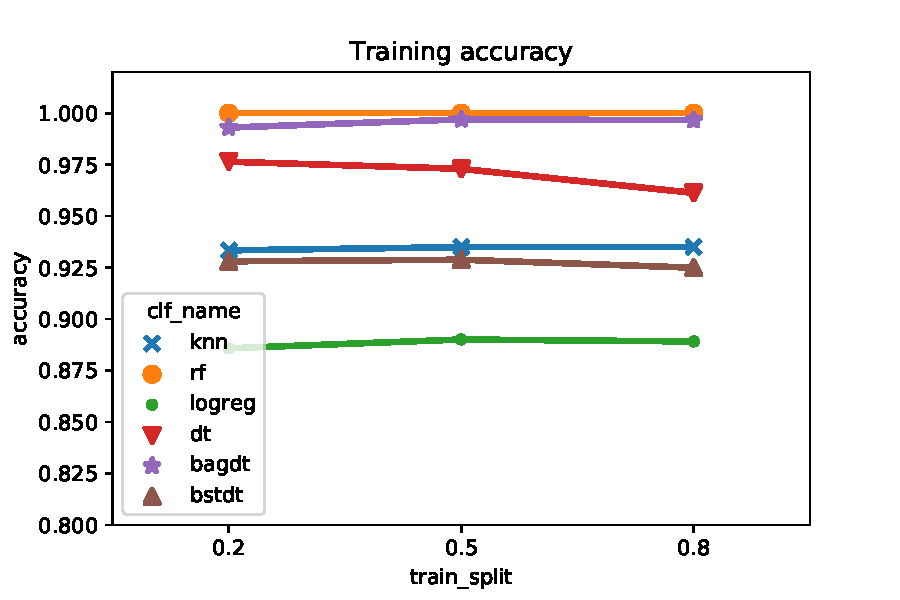
\includegraphics[width=\textwidth]{tr_acc_by_clf_trainsplit}
					\caption{Training accuracy}
					\label{fig:perf_by_trainsplit_tr}
				\end{subfigure}
				\begin{subfigure}{.5\textwidth}
					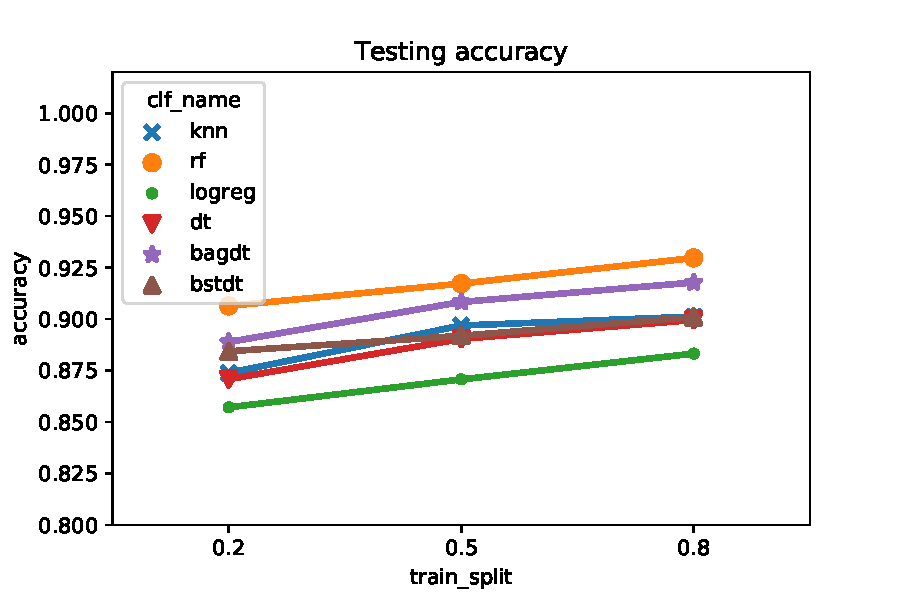
\includegraphics[width=\textwidth]{te_acc_by_clf_trainsplit}
					\caption{Testing accuracy}
					\label{fig:perf_by_trainsplit_te}
				\end{subfigure}
			\caption{Training and testing accuracy by train split, averaged over problems and shuffles}
			\label{fig:perf_by_trainsplit}
			\end{figure}
		
		\subsection{Overall Classifier Performance}
			% Overall average results of clfs on datasets
			\begin{table}[h]
				\caption{Classifier testing accuracy by problem, averaged over shuffles (0.8 train split)}
				\begin{tabular}{lrrrrr}
					\toprule
					Classifier & WDBC & INCOME & IRIS & COVTYPE & LETTER \\
					\midrule
					bagdt  & .968 &   .833 & .944 &    .971 &   .873 \\
					bstdt  & .968 &   .840 & .956 &    .971 &   .771 \\
					dt     & .953 &   .799 & .956 &    .970 &   .820 \\
					knn    & .950 &   .757 & .933 &    .967 &   \textbf{.899} \\
					logreg & .968 &   .792 & \textbf{.967} &    .968 &   .721 \\
					rf     & \textbf{.982} &   \textbf{.848} & .944 &    \textbf{.976} &   .897 \\
					\bottomrule
				\end{tabular}
			\end{table}
		
			% Overall average results of clfs, sorted
			\begin{table}[h]
				\caption{Ranked classifiers by testing accuracy, averaged over problems and shuffles (0.8 train split)}
				\begin{tabular}{lr}
					\toprule
					{Classifier} & Accuracy \\
					\midrule
					rf     &     .930 \\
					bagdt  &     .918 \\
					knn    &     .901 \\
					bstdt  &     .901 \\
					dt     &     .900 \\
					logreg &     .883 \\
					\bottomrule
				\end{tabular}
			\end{table}
	
	\section{Conclusion}
	
	\section{Bonus Points}
	
	\section{References}
	
	
	
	
	
	
	
	\newpage
	
	\appendix
	\section*{Appendix A.}
	\label{app:theorem}
	
	
	
	\vskip 0.2in
	\bibliography{sample}
	
\end{document}